\documentclass[border=10pt]{standalone}
\usepackage[svgnames]{xcolor}
\usepackage{amsmath}
\usepackage{pgfplots}
\pgfplotsset{compat=newest}
\usepackage[sfdefault]{FiraSans}
\usepackage{FiraMono}
\renewcommand*\familydefault{\sfdefault}
\begin{document}
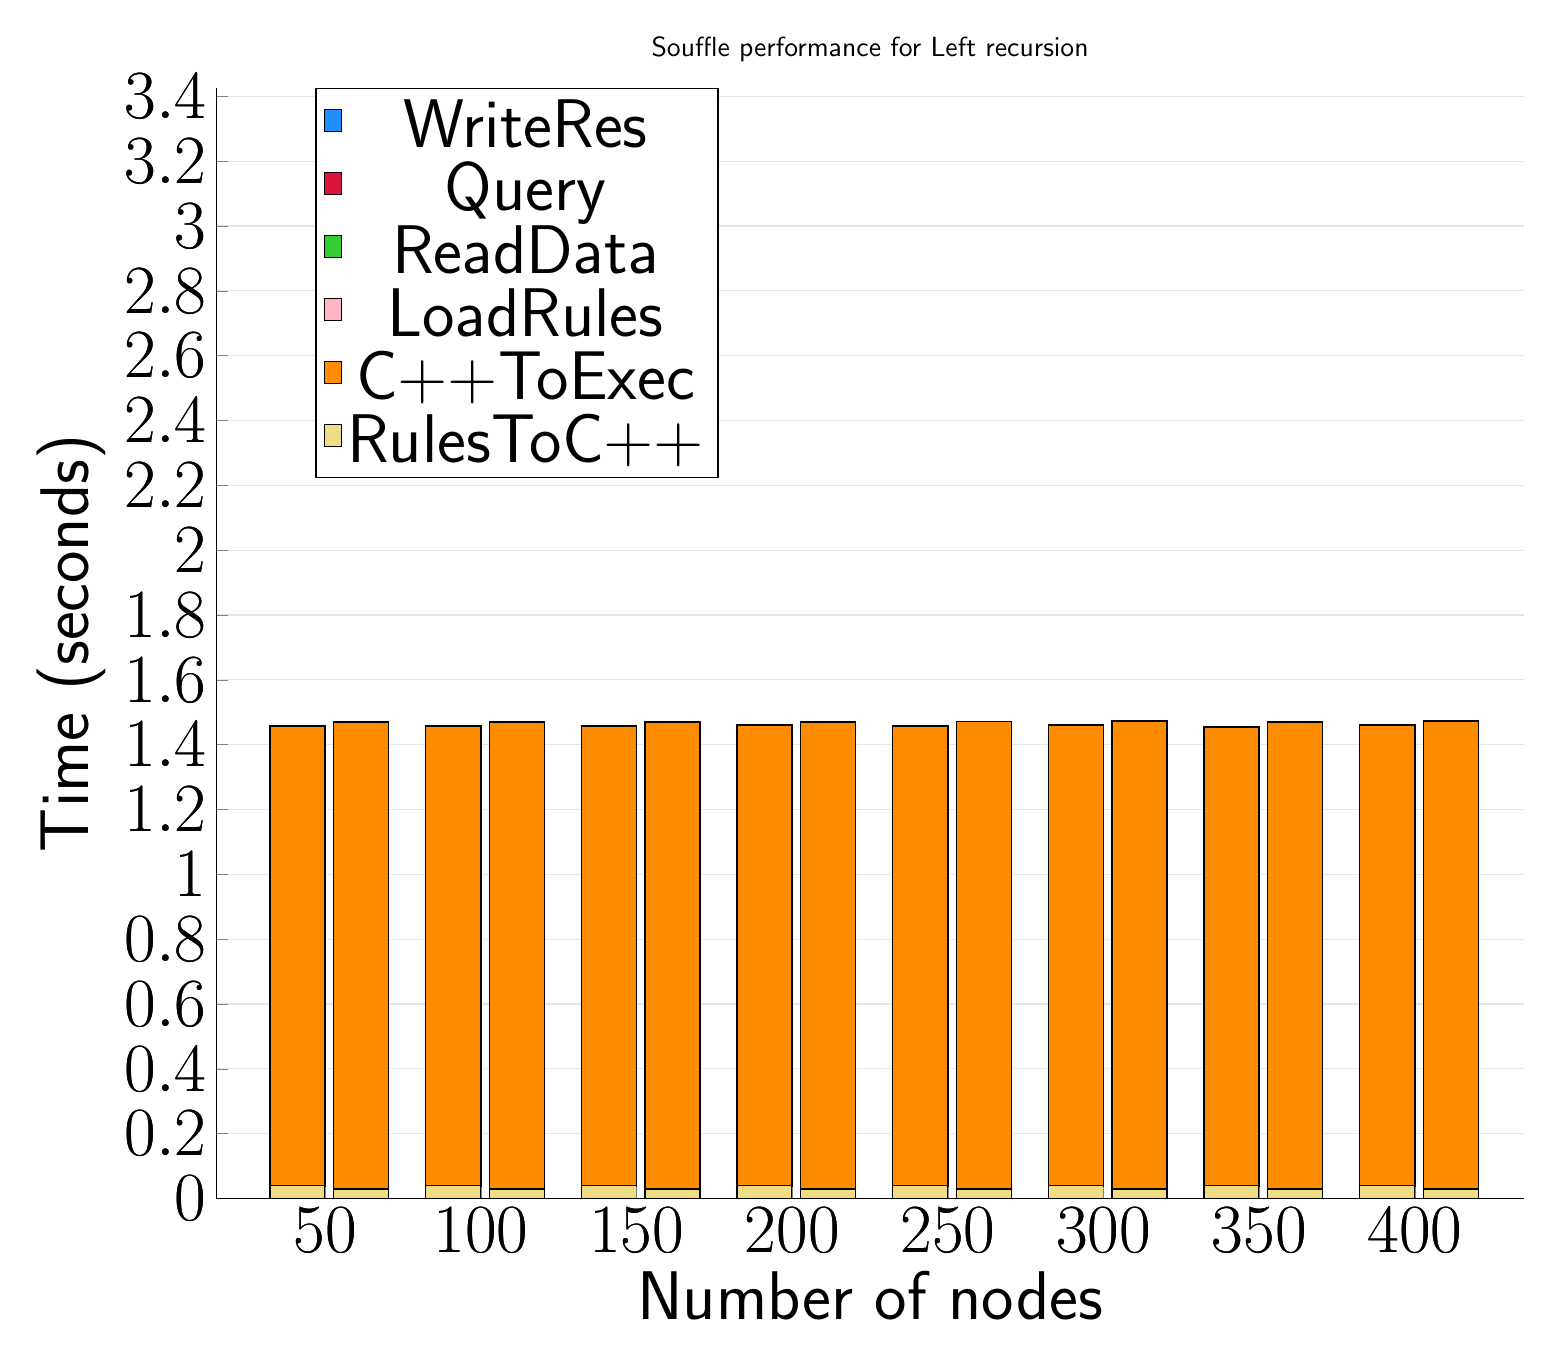
\begin{tikzpicture}
	\begin{axis}[
			ybar stacked,
			title={Souffle performance for Left recursion},
			bar shift=-10pt,
			width=1.5\textwidth,
			bar width=0.7cm,
			ymajorgrids, tick align=inside,
			major grid style={draw=gray!20},
			xtick=data,
			ymin=0, ymax=3.4260000705718996,
			axis x line*=bottom,
			axis y line*=left,
			enlarge x limits=0.1,
			legend style={
					at={(0.23, 1)},
					anchor=north,
					legend columns=1,
					font=\Huge,
				},
			ylabel={Time (seconds)},
			xlabel={Number of nodes},
			label style={font=\Huge},
			tick label style={font=\Huge},
		]
		\addlegendimage{fill=DodgerBlue, draw=black, line width=0.2pt}
		\addlegendentry{WriteRes}
		\addlegendimage{fill=Crimson, draw=black, line width=0.2pt}
		\addlegendentry{Query}
		\addlegendimage{fill=LimeGreen, draw=black, line width=0.2pt}
		\addlegendentry{ReadData}
		\addlegendimage{fill=LightPink, draw=black, line width=0.2pt}
		\addlegendentry{LoadRules}
		\addlegendimage{fill=DarkOrange, draw=black, line width=0.2pt}
		\addlegendentry{C++ToExec}
		\addlegendimage{fill=LightGoldenrod, draw=black, line width=0.2pt}
		\addlegendentry{RulesToC++}
		\addplot +[fill=LightGoldenrod, draw=black, line width=0.5pt] coordinates {
				(50, 0.04000003337860107)
				(100, 0.04100003242492676)
				(150, 0.039999985694885255)
				(200, 0.039999985694885255)
				(250, 0.04000000953674317)
				(300, 0.04000000953674317)
				(350, 0.039999985694885255)
				(400, 0.040999984741210936)
			};
		\addplot +[fill=DarkOrange, draw=black, line width=0.5pt] coordinates {
				(50, 1.4169999837875367)
				(100, 1.415999984741211)
				(150, 1.4170000314712525)
				(200, 1.4200000047683716)
				(250, 1.4180000066757201)
				(300, 1.419000005722046)
				(350, 1.4149999856948852)
				(400, 1.4180000066757201)
			};
		\addplot +[fill=LightPink, draw=black, line width=0.5pt] coordinates {
				(50, 0.0001233208)
				(100, 0.0001127332)
				(150, 0.00011290829999999999)
				(200, 9.82583e-05)
				(250, 0.0001235833)
				(300, 0.00010100839999999998)
				(350, 0.0001005873)
				(400, 9.5275e-05)
			};
		\addplot +[fill=LimeGreen, draw=black, line width=0.5pt] coordinates {
				(50, 0.0003413708)
				(100, 0.00045633740000000005)
				(150, 0.0005559707)
				(200, 0.0006385499000000001)
				(250, 0.0007817542)
				(300, 0.0008612455999999999)
				(350, 0.0009292500000000002)
				(400, 0.0010528156000000001)
			};
		\addplot +[fill=Crimson, draw=black, line width=0.5pt] coordinates {
				(50, 0.0)
				(100, 7.54418e-05)
				(150, 0.0001384583)
				(200, 0.0001844664)
				(250, 0.00024421219999999996)
				(300, 0.0002735166)
				(350, 0.00031521669999999997)
				(400, 0.000365725)
			};
		\addplot +[fill=DodgerBlue, draw=black, line width=0.5pt] coordinates {
				(50, 0.0002393207)
				(100, 0.00026037909999999996)
				(150, 0.0002816)
				(200, 0.0002987708)
				(250, 0.0003364916)
				(300, 0.0004350872999999999)
				(350, 0.0003609167)
				(400, 0.00039758320000000003)
			};
	\end{axis}
	\begin{axis}[
			ybar stacked,
			bar shift=13pt,
			width=1.5\textwidth,
			bar width=0.7cm,
			ymajorgrids, tick align=inside,
			major grid style={draw=none},
			xtick=data,
			ymin=0, ymax=3.4260000705718996,
			axis x line*=none,
			axis y line*=none,
			enlarge x limits=0.1,
			label style={font=\Huge},
			tick label style={font=\Huge},
		]
		\addplot +[fill=LightGoldenrod, draw=black, line width=0.5pt] coordinates {
				(50, 0.030000000000000006)
				(100, 0.030000000000000006)
				(150, 0.030000000000000006)
				(200, 0.030000000000000006)
				(250, 0.030000000000000006)
				(300, 0.030000000000000006)
				(350, 0.030000000000000006)
				(400, 0.030000000000000006)
			};
		\addplot +[fill=DarkOrange, draw=black, line width=0.5pt] coordinates {
				(50, 1.4389999999999996)
				(100, 1.4399999999999997)
				(150, 1.44)
				(200, 1.44)
				(250, 1.4409999999999996)
				(300, 1.4409999999999998)
				(350, 1.4379999999999997)
				(400, 1.4419999999999997)
			};
		\addplot +[fill=LightPink, draw=black, line width=0.5pt] coordinates {
				(50, 0.0001226)
				(100, 0.00011169999999999999)
				(150, 0.0001121)
				(200, 9.74e-05)
				(250, 0.0001225)
				(300, 0.0001003)
				(350, 0.0001)
				(400, 9.47e-05)
			};
		\addplot +[fill=LimeGreen, draw=black, line width=0.5pt] coordinates {
				(50, 0.0003406)
				(100, 0.0004554)
				(150, 0.0005556000000000001)
				(200, 0.0006376999999999999)
				(250, 0.0007809)
				(300, 0.0008602)
				(350, 0.0009284)
				(400, 0.001052)
			};
		\addplot +[fill=Crimson, draw=black, line width=0.5pt] coordinates {
				(50, 0.0)
				(100, 7.510000000000001e-05)
				(150, 0.0001379)
				(200, 0.00018390000000000002)
				(250, 0.00024370000000000004)
				(300, 0.00027299999999999997)
				(350, 0.00031469999999999995)
				(400, 0.0003656)
			};
		\addplot +[fill=DodgerBlue, draw=black, line width=0.5pt] coordinates {
				(50, 0.0002386)
				(100, 0.0002595)
				(150, 0.00028069999999999994)
				(200, 0.0002979)
				(250, 0.00033580000000000003)
				(300, 0.00034619999999999996)
				(350, 0.0003601)
				(400, 0.00039700000000000005)
			};
	\end{axis}
\end{tikzpicture}

\end{document}
